% !TEX program = lualatex
%==============================================================================
%  Intra-Plane Coupling in the Multiple Scattering of Elastodynamic Waves
%  in a Depth-Stratified Medium.
%
%  Self-contained LuaLaTeX source. Compile with:
%      latexmk -lualatex EwaldIntraPlanePropagator.tex
%  or, manually, two passes of:
%      lualatex EwaldIntraPlanePropagator.tex
%==============================================================================
\documentclass[11pt,a4paper]{article}

% --- LuaLaTeX font handling -------------------------------------------------
\usepackage{fontspec}
\setmainfont{Latin Modern Roman}

% --- Mathematics ------------------------------------------------------------
\usepackage{amsmath}
\usepackage{amssymb}
\usepackage{mathtools}

% --- Layout and typography --------------------------------------------------
\usepackage[margin=1in]{geometry}
\usepackage{microtype}
\usepackage{xcolor}
\usepackage{booktabs}

% --- Graphics ---------------------------------------------------------------
\usepackage{tikz}
\usetikzlibrary{decorations.pathmorphing, arrows.meta}

% --- Hyperlinks (loaded late) -----------------------------------------------
\usepackage[colorlinks=true,
            linkcolor=blue!55!black,
            citecolor=blue!55!black,
            urlcolor=blue!55!black]{hyperref}
\hypersetup{
  pdftitle={Intra-Plane Coupling in Elastodynamic Multiple Scattering},
  pdfauthor={Tod Nestor}
}

% --- Macros -----------------------------------------------------------------
\DeclareMathOperator{\erfc}{erfc}
\newcommand{\rd}{\mathrm{d}}
\newcommand{\ii}{\mathrm{i}}
\newcommand{\Imm}{\operatorname{Im}}
\newcommand{\kpar}{\mathbf{k}_{\parallel}}
\newcommand{\vr}{\mathbf{r}}
\newcommand{\vR}{\mathbf{R}}
\newcommand{\vG}{\mathbf{G}}
\newcommand{\brho}{\boldsymbol{\rho}}
\newcommand{\Lat}{\Lambda}
\newcommand{\dLat}{\Lambda^{\ast}}
\newcommand{\kzG}{k_{z,\vG}}

\title{\bfseries Intra-Plane Coupling in the Multiple Scattering of
Elastodynamic Waves in a Depth-Stratified Medium\\[4pt]
\large Plane-Wave Propagators, Conditional Convergence, and Ewald Summation}
\author{Tod Nestor}
\date{16 June 2026}

\begin{document}
\maketitle

\begin{abstract}
The Green's tensor of a depth-stratified elastodynamic medium admits a partial-wave
(plane-wave) expansion in which the depth-direction wavenumber of each constituent wave
is fixed, through the dispersion relation, by the frequency, the local wavespeed of that
partial wave, and the horizontal wavenumber. Used as an inter-site propagator for
multiple-scattering sites, this representation is optimal when the sites lie at different
depths: the evanescent spectrum supplies an exponential convergence factor whose rate
grows with the depth separation. The same representation fails to converge when two sites
share a depth, because that exponential damping disappears. This note records why, and
then develops the standard cure for the intra-plane (equal-depth) coupling: Ewald
summation of the Bloch-periodic lattice sum. We present the method in the language of
analytic number theory, where it is the theta-splitting argument used to continue an
Epstein zeta function, give the explicit real-space and reciprocal-space halves with their
Gaussian convergence factors, and reduce the elastodynamic tensor problem to two scalar
Helmholtz lattice sums by an exact operator identity. Finally we derive the SH and P/SV
traction kernels, the displacement-traction partial-wave system whose continuity across
interfaces and scatterer surfaces closes the multiple-scattering problem, and check them
against the Rayleigh secular equation. A closing section applies the convergence theory to a
space-filling grid of scatterers: the coupling splits into the same-depth near field, an
interplane specular response carried by the Kennett recursion, and an interplane
side-scattering term that the same evanescent scale confines to the nearest diagonal
neighbours. Same-depth and interplane near fields then merge into a single first-shell
real-space stencil over a global spectral propagator.
\end{abstract}

\bigskip
\noindent\textbf{Companion series.}\enspace{\small\itshape One of a companion series on elastic
multiple scattering from cubic heterogeneities on a depth-stratified background, the T-matrix
programme $T=T_0(I-G_0T_0)^{-1}$: \textbf{(I)}~the stratified inter-site propagator, the
same-depth convergence theory, the SH and P/SV traction kernels, interplane side scattering and
the first-shell near stencil (\texttt{EwaldIntraPlanePropagator}); \textbf{(II)}~the
contrast-source volume integral equation and the CG-FFT / seismic grid T-matrix lineage
(\texttt{ContrastSourceVIE}); \textbf{(III)}~the directional partial-wave sweep matvec and the
Krylov multiple-scattering solve (\texttt{DirectionalSweepSolver}); with the empirical companion
\texttt{RQ1\_Planar\_Decomposition\_Proposal}. This is note~(I).}

\tableofcontents
\bigskip

%==============================================================================
\section{The stratified Green's tensor and its partial-wave expansion}
%==============================================================================

Let the elastic properties of the medium (density $\rho$ and the isotropic moduli,
equivalently the compressional and shear speeds $\alpha$ and $\beta$) depend only on the
depth coordinate $z$, and be invariant under translations in the horizontal plane. That
horizontal homogeneity is what permits a Fourier transform over the horizontal coordinates
$\brho=(x,y)$ and time $t$, reducing the full three-dimensional problem to a family of
one-dimensional (in depth) problems, one for each horizontal wavevector $\kpar=(k_x,k_y)$
and frequency $\omega$. The Green's tensor $G_{ij}(\vr,\vr';t)$ is expanded over these
plane waves, each carrying a factor $\exp[\ii(\kpar\cdot\brho-\omega t)]$.

Within any locally homogeneous region the field decomposes into upgoing and downgoing
partial waves: compressional (P) and vertically polarised shear (SV), together with the
horizontally polarised shear (SH) waves that decouple. For a partial wave of local speed
$c$ the depth-direction wavenumber follows from the dispersion relation
\begin{equation}
\label{eq:disp}
k_z(c) \;=\; \sqrt{\dfrac{\omega^{2}}{c^{2}} - k_x^{2} - k_y^{2}},
\qquad c\in\{\alpha,\beta\}, \qquad \Imm k_z \ge 0 .
\end{equation}
The total wavevector has fixed magnitude $\omega/c$; the vertical component $k_z$ is
whatever remains after the horizontal part is removed. Two partial waves at the same
$\omega$ and $\kpar$ therefore carry \emph{different} vertical wavenumbers,
\begin{align}
\label{eq:PSdisp}
k_z^{(\alpha)} &= \sqrt{\omega^{2}/\alpha^{2}-k_\parallel^{2}} \quad\text{(P)},
&
k_z^{(\beta)} &= \sqrt{\omega^{2}/\beta^{2}-k_\parallel^{2}} \quad\text{(S)},
\end{align}
with $k_\parallel=|\kpar|$. In ray-parameter form, with horizontal slowness $p=k_\parallel/\omega$
and vertical slownesses $q_c=\sqrt{1/c^{2}-p^{2}}$, one has $k_z=\omega\,q_c$.

The branch in \eqref{eq:disp} carries the essential physics. When $\omega^2/c^2>k_\parallel^2$
the wave propagates obliquely ($k_z$ real); when $\omega^2/c^2<k_\parallel^2$ it is evanescent
($k_z$ imaginary), decaying with depth. The evanescent branch is what carries head waves,
post-critical reflections, and interface and surface modes. The whole stratification enters
diagonally in $(\kpar,\omega)$: reflection and transmission from the layering appear as
coefficients multiplying the up- and downgoing partial waves, stitched across interfaces by
continuity of displacement and traction.

%==============================================================================
\section{The inter-site propagator and depth-separation convergence}
%==============================================================================

For a homogeneous reference medium the scalar building block of the propagator is the
outgoing Helmholtz kernel, and its plane-wave (Weyl, or Sommerfeld) representation is
\begin{equation}
\label{eq:weyl}
\frac{e^{\ii\kappa r}}{4\pi r}
\;=\;
\frac{\ii}{8\pi^{2}}\int_{\mathbb{R}^{2}}\frac{\rd^{2}\kpar}{k_z}\,
e^{\,\ii(\kpar\cdot\brho + k_z\lvert z\rvert)},
\qquad \kappa=\omega/c,\quad k_z=\sqrt{\kappa^{2}-k_\parallel^{2}}, \quad \Imm k_z\ge 0 .
\end{equation}
The depth dependence sits entirely in $e^{\ii k_z|z-z'|}$. Past the radiative cone,
$k_\parallel>\kappa$, we have $k_z=\ii\kappa_\perp$ with $\kappa_\perp=\sqrt{k_\parallel^{2}-\kappa^{2}}>0$,
and that factor becomes a real exponential decay,
\begin{equation}
e^{\ii k_z|\Delta z|}=e^{-\kappa_\perp|\Delta z|}, \qquad \Delta z = z-z'.
\end{equation}
This is the only mechanism that tames the large-$k_\parallel$ tail of the spectral integral, or,
for a periodic arrangement of sites, of the lattice sum. Examine that tail. At large
$k_\parallel$, $1/k_z\sim 1/(\ii k_\parallel)$, the two-dimensional measure contributes
$k_\parallel\,\rd k_\parallel$, and the kernel contributes $e^{-k_\parallel|\Delta z|}$, so
\begin{equation}
\label{eq:tail}
\int^{\infty}\! k_\parallel\,\rd k_\parallel \;\frac{1}{k_\parallel}\,e^{-k_\parallel|\Delta z|}
\;=\;
\int^{\infty}\!\rd k_\parallel\,e^{-k_\parallel|\Delta z|}
\;=\;
\frac{1}{|\Delta z|}.
\end{equation}
The radial integral is finite if and only if $\Delta z\neq 0$, and it converges \emph{faster
the larger $|\Delta z|$ is}. This is precisely why the partial-wave representation is the
optimal inter-site propagator across depths: the stratification is already diagonal in
$(\kpar,\omega)$, and the evanescent spectrum self-truncates exponentially at a rate set by
the depth offset. Two sites at different depths, even directly above one another, are joined
by an absolutely and rapidly convergent sum.

%==============================================================================
\section{Breakdown of the representation at equal depth}
%==============================================================================

Set $\Delta z=0$. The damping factor becomes $e^{-\kappa_\perp\cdot 0}=1$, the high-$k_\parallel$
evanescent waves are no longer suppressed, and \eqref{eq:tail} collapses to
$\int^{\infty}\rd k_\parallel$, which diverges. Only the horizontal phase
$e^{\ii\kpar\cdot\Delta\brho}$ remains:
\begin{itemize}
  \item \textbf{Distinct in-plane sites} ($\Delta\brho\neq 0,\ \Delta z=0$): the sum is only
  \emph{conditionally} convergent. Its value depends on the order of summation, and as a
  lattice sum it is the classic non-convergent structure constant.
  \item \textbf{Coincident sites} ($\Delta\brho=0,\ \Delta z=0$): the sum diverges outright,
  which is simply the near-field singularity of the Green's tensor appearing unmasked, since
  that singularity \emph{is} the large-$k_\parallel$ evanescent content.
\end{itemize}
It is worth stressing that the physical propagator between two distinct equal-depth sites is
perfectly finite. What fails is this particular representation, not the quantity it
represents. The evanescent expansion converges to the correct value everywhere off the plane
and loses convergence on it.

\begin{figure}[h]
\centering
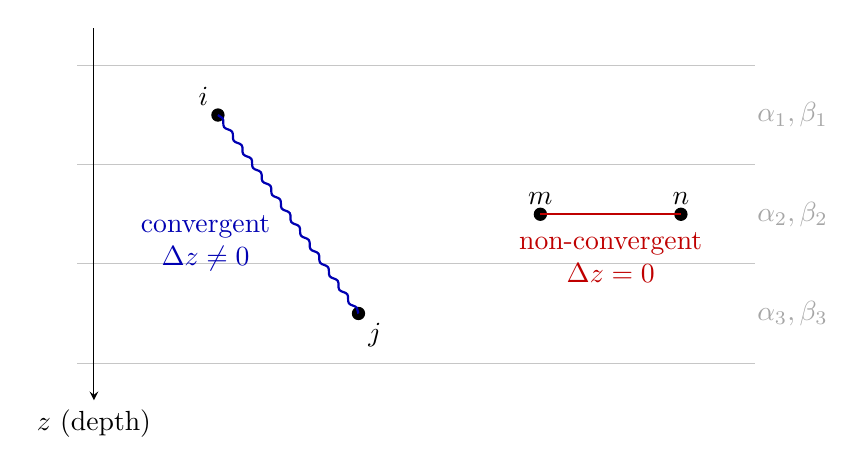
\begin{tikzpicture}[>=stealth, scale=1.05]
  % layer boundaries
  \foreach \y in {0,-1.2,-2.4,-3.6}{\draw[gray!45] (-0.2,\y) -- (8.0,\y);}
  \node[gray!70] at (8.45,-0.6) {$\alpha_1,\beta_1$};
  \node[gray!70] at (8.45,-1.8) {$\alpha_2,\beta_2$};
  \node[gray!70] at (8.45,-3.0) {$\alpha_3,\beta_3$};
  % depth axis
  \draw[->] (0.0,0.45) -- (0.0,-4.05) node[below] {$z$ (depth)};
  % sites at different depths -> convergent
  \filldraw[black] (1.5,-0.6) circle (2.1pt) node[above left] {$i$};
  \filldraw[black] (3.2,-3.0) circle (2.1pt) node[below right] {$j$};
  \draw[blue!70!black, thick, decorate,
        decoration={snake, amplitude=0.7pt, segment length=6pt}]
        (1.5,-0.6) -- (3.2,-3.0);
  \node[blue!70!black, align=center] at (1.35,-2.15)
        {convergent\\ $\Delta z\neq 0$};
  % sites at same depth -> non-convergent
  \filldraw[black] (5.4,-1.8) circle (2.1pt) node[above] {$m$};
  \filldraw[black] (7.1,-1.8) circle (2.1pt) node[above] {$n$};
  \draw[red!75!black, thick] (5.4,-1.8) -- (7.1,-1.8);
  \node[red!75!black, align=center] at (6.25,-2.32)
        {non-convergent\\ $\Delta z = 0$};
\end{tikzpicture}
\caption{The plane-wave inter-site propagator. A vertical separation $\Delta z\neq 0$
supplies the evanescent damping $e^{-\kappa_\perp|\Delta z|}$ that makes the spectral sum
converge (blue). Sites sharing a depth, $\Delta z = 0$, lose that factor and the
representation ceases to converge (red).}
\end{figure}

This is the same split that layered multiple-scattering theory lives with, and the
elastodynamic counterpart of the layer-KKR / LEED structure-constant problem of
Korringa, Kohn and Rostoker, of Kambe, and of Pendry and Modinos: a plane-wave
(reciprocal-space) propagator between sites in different planes, and a separate real-space
construction, or an Ewald resummation, for sites within one plane.

%==============================================================================
\section{Intra-plane coupling by Ewald summation}
%==============================================================================

\subsection{The object, in analytic terms}

Fix a two-dimensional Bravais lattice $\Lat\subset\mathbb{R}^{2}$ of scatterer positions in
the plane, a Bloch character $\kpar$, and a wavenumber $\kappa=\omega/c$. The intra-plane
propagator is the quasi-periodic Helmholtz lattice sum
\begin{equation}
\label{eq:bloch}
\mathcal{G}(\vr)
\;=\;
\sum_{\vR\in\Lat}\frac{e^{\ii\kappa|\vr-\vR|}}{4\pi|\vr-\vR|}\;
e^{\ii\kpar\cdot\vR}.
\end{equation}
The two representations of \S2--\S3 are its two faces: \eqref{eq:bloch} is the real-space
form (terms $\sim 1/|\vR|$, conditionally convergent), and its Poisson dual over the
reciprocal lattice $\dLat$ is the plane-wave form (terms $\sim 1/\kzG$, convergent off the
plane, divergent on it). On the plane $z=0$ neither series converges absolutely. The task is
purely analytic: assign $\mathcal{G}$ its correct finite value and compute it efficiently.

\subsection{The Gaussian representation and the split}

Write each term through the Gaussian (Mellin, or heat-kernel) representation
\begin{equation}
\label{eq:gaussrep}
\frac{e^{\ii\kappa R}}{4\pi R}
\;=\;
\frac{1}{2\pi^{3/2}}\int_{0}^{\infty}
\exp\!\Big(-R^{2}\xi^{2}+\frac{\kappa^{2}}{4\xi^{2}}\Big)\,\rd\xi,
\end{equation}
where the lower endpoint is made convergent by a slight rotation of the contour (for
$\kappa\to 0$ this is exactly the $\Gamma$-function integral behind $\zeta$). Now cut the
$\xi$-integral at an arbitrary $\eta>0$ and sum:
\begin{equation}
\mathcal{G}=\mathcal{G}^{(1)}+\mathcal{G}^{(2)},
\qquad
\mathcal{G}^{(1)}\!\leftrightarrow\!\int_{\eta}^{\infty},
\qquad
\mathcal{G}^{(2)}\!\leftrightarrow\!\int_{0}^{\eta}.
\end{equation}
The upper piece keeps the strong Gaussian cutoff $e^{-R^{2}\xi^{2}}$ and is summed in real
space; the lower piece carries the long-range tail and is Poisson-transformed to the dual
lattice. Because the Gaussian is self-dual under the Fourier transform, the dual lattice also
sees a Gaussian, so both halves converge at Gaussian rate. The split point $\eta$ is free and
the total is exactly $\eta$-independent: that invariance is the practical numerical check, and
$\eta$ is tuned to balance the two sums, typically $\eta\approx\sqrt{\pi}/\sqrt{A}$ with $A$
the area of the unit cell.

\subsection{Real-space half}

Carrying out $\int_\eta^\infty$ term by term yields error functions,
\begin{equation}
\label{eq:real}
\boxed{\;
\mathcal{G}^{(1)}(\vr)
=
\frac{1}{8\pi}\sum_{\vR\in\Lat}\frac{e^{\ii\kpar\cdot\vR}}{|\vr-\vR|}
\sum_{s=\pm 1}
e^{\,s\,\ii\kappa|\vr-\vR|}\,
\erfc\!\Big(|\vr-\vR|\,\eta+s\,\frac{\ii\kappa}{2\eta}\Big)\; }
\end{equation}
For large $|\vR|$ the argument of each $\erfc$ tends to $+\infty$, so the term decays like
$e^{-\eta^{2}|\vR|^{2}}$. The real-space sum is absolutely and Gaussian-fast convergent.

\subsection{Reciprocal-space half}

Poisson summation of $\int_0^\eta$ over $\Lat$ (the calculation is in the appendix) gives a
sum over $\dLat$. Specialised to the plane $z=0$, where the bare spectral sum failed, it is
\begin{equation}
\label{eq:recip}
\boxed{\;
\mathcal{G}^{(2)}(\brho,0)
=
\frac{\ii}{2A}\sum_{\vG\in\dLat}
\frac{e^{\ii(\kpar+\vG)\cdot\brho}}{\kzG}\,
\erfc\!\Big(\frac{\kzG}{2\ii\eta}\Big),
\qquad
\kzG=\sqrt{\kappa^{2}-|\kpar+\vG|^{2}},\ \ \Imm\kzG\ge 0. \;}
\end{equation}
For evanescent orders, $\kzG=\ii\sqrt{|\kpar+\vG|^{2}-\kappa^{2}}$, the $\erfc$ argument is
real and positive and the term decays like $e^{-(|\kpar+\vG|^{2}-\kappa^{2})/4\eta^{2}}$,
Gaussian in $|\vG|$. The finitely many propagating orders ($|\kpar+\vG|<\kappa$) give an
$\erfc$ of imaginary argument and are evaluated directly. Letting $\eta\to\infty$ sends
$\erfc\to 1$ and recovers the bare, divergent spectral sum
$\tfrac{\ii}{2A}\sum_{\vG}\kzG^{-1}e^{\ii(\kpar+\vG)\cdot\brho}$; the factor
$\erfc(\kzG/2\ii\eta)$ is exactly the regulator that the equal-depth configuration was
missing.

\begin{table}[h]
\centering
\renewcommand{\arraystretch}{1.3}
\begin{tabular}{@{}llll@{}}
\toprule
Half & Summed over & Convergence factor & Decay rate \\
\midrule
real-space, \eqref{eq:real} & direct lattice $\Lat$ &
$\erfc(|\vR|\eta+\tfrac{\ii\kappa}{2\eta})$ & $e^{-\eta^{2}|\vR|^{2}}$ \\
reciprocal-space, \eqref{eq:recip} & dual lattice $\dLat$ &
$\erfc(\kzG/2\ii\eta)$ & $e^{-|\kpar+\vG|^{2}/4\eta^{2}}$ \\
\bottomrule
\end{tabular}
\caption{The two halves of the Ewald-summed intra-plane propagator. Both are Gaussian-fast;
their sum is independent of $\eta$.}
\end{table}

\subsection{Why a mathematician already knows this}

Equations \eqref{eq:gaussrep}--\eqref{eq:recip} are the theta-splitting argument that
continues an Epstein zeta function and proves its functional equation. The Gaussian integral
is the Mellin representation; cutting at $\eta$ is splitting the Mellin integral at a chosen
point; Poisson summation of the Gaussian is the Jacobi imaginary transformation
$\theta(1/t)=t^{1/2}\theta(t)$. Read ``Ewald parameter'' as ``the cut in the theta integral,''
and read convergence at $z=0$ as nothing more mysterious than the analytic continuation of
$\sum_{\vR}Q(\vR)^{-s}$ past its abscissa of convergence. The mechanism is the self-duality
of the Gaussian under the Fourier transform: it is the unique regulator that tames a lattice
and its dual at once.

\subsection{A finite heterogeneity: zero-padding into a corner}

Sections \S4.1--\S4.4 compute the \emph{periodic} structure constant: the reciprocal sum over
$\dLat$ is the field of an infinite array that tiles the plane. A real heterogeneity is not
that. It is a finite lateral patch of cells embedded in the layered background, and against a
finite patch the periodic reciprocal sum is the wrong operator, because it couples the patch to
spurious periodic images of itself. The fast Fourier transform that evaluates the far half is
itself intrinsically a \emph{circular} convolution: it wraps a cell at one edge of the box onto
a cell at the opposite edge.

The cure is zero-padding, and its geometry is a corner (Figure~\ref{fig:padding}). Embed the
patch, of lateral extent $L$, in a computational box of side at least $2L$, so that the
scatterers occupy one corner and the remainder holds none. The circular convolution over the
padded box, read back on the patch, then equals the \emph{linear} (aperiodic) convolution
exactly: every wraparound image falls in the empty padding, a gap of at least $L$ from the real
cells, and never reaches them. For a finite region the periodic structure constant of \S4.4 is
thereby replaced by the zero-padded transform of the patch in a corner.

\begin{figure}[h]
\centering
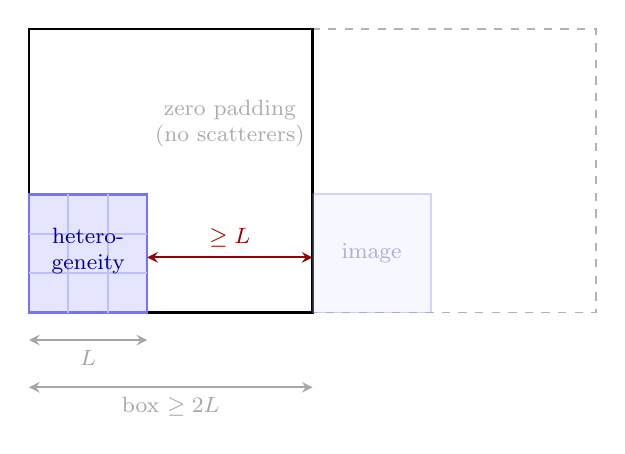
\begin{tikzpicture}[>=stealth, line width=0.7pt]
  \draw[black, line width=1pt] (0,0) rectangle (3.6,3.6);
  \fill[blue!10] (0,0) rectangle (1.5,1.5);
  \draw[blue!55, line width=0.9pt] (0,0) rectangle (1.5,1.5);
  \foreach \i in {0.5,1.0}{\draw[blue!25] (\i,0)--(\i,1.5); \draw[blue!25] (0,\i)--(1.5,\i);}
  \node[blue!60!black, align=center] at (0.75,0.78)
        {\footnotesize hetero-\\[-2.5pt]\footnotesize geneity};
  \node[gray!65, align=center] at (2.55,2.4)
        {\footnotesize zero padding\\[-2.5pt]\footnotesize (no scatterers)};
  \begin{scope}[opacity=0.30]
    \draw[black, dashed] (3.6,0) rectangle (7.2,3.6);
    \fill[blue!10] (3.6,0) rectangle (5.1,1.5);
    \draw[blue!55] (3.6,0) rectangle (5.1,1.5);
    \node[blue!60!black] at (4.35,0.75) {\footnotesize image};
  \end{scope}
  \draw[<->, red!60!black] (1.5,0.7)--(3.6,0.7)
        node[midway, above, red!60!black]{\footnotesize $\ge L$};
  \draw[<->, gray!70] (0,-0.35)--(1.5,-0.35) node[midway, below]{\footnotesize $L$};
  \draw[<->, gray!70] (0,-0.95)--(3.6,-0.95) node[midway, below]{\footnotesize box $\ge 2L$};
\end{tikzpicture}
\caption{Zero-padded embedding of a finite heterogeneity for the aperiodic transform. The patch
of lateral extent $L$ sits in one corner of a box of side at least $2L$, the remainder carrying
no scatterers. The circular convolution the FFT performs then equals the linear, aperiodic
convolution on the patch, because the nearest periodic image (dashed) is held at least a gap $L$
away in the empty padding and never reaches a real cell. Only the reciprocal half changes; the
real-space near stencil is untouched.}
\label{fig:padding}
\end{figure}

Two points make this the natural update rather than a patch on the method. First, only the
reciprocal (far) half changes: the real-space near half of \S4.3, the first-shell stencil of
\S7.4, is local and periodicity-agnostic and is untouched. Second, because the patch is small
and localised, the transform is taken over the box alone, while the infinite layered background
outside it is carried analytically by the propagator, with no discretisation reaching to
infinity and no absorbing boundary. The cost is a box doubled per lateral dimension, four times
the area and transform work in the plane, in exchange for periodic images that contribute
exactly zero. This is the exact counterpart of re-imposing periodicity through a large supercell
with absorption: the padding removes the images without approximation.

%==============================================================================
\section{Reducing the elastic tensor to scalar lattice sums}
%==============================================================================

One does not need a separate dyadic theory. In a homogeneous reference medium the
elastodynamic Green's tensor is an exact, fixed second-order differential operator applied
to two scalar Helmholtz kernels, one at the P-number $\kappa_P=\omega/\alpha$ and one at the
S-number $\kappa_S=\omega/\beta$:
\begin{equation}
\label{eq:opident}
G_{ij}(\vr)
=
\frac{1}{\rho\omega^{2}}
\Big[\big(\kappa_S^{2}\,\delta_{ij}+\partial_i\partial_j\big)\,g_S(\vr)
-\partial_i\partial_j\,g_P(\vr)\Big],
\qquad
g_c(\vr)=\frac{e^{\ii\kappa_c r}}{4\pi r}.
\end{equation}
This identity is exact, not asymptotic. In Fourier space the longitudinal and transverse
projectors make the $1/k^{2}$ near-field pieces cancel identically, so \eqref{eq:opident}
already contains the full near field. Because $\partial_i\partial_j$ acts on the field point
while the lattice sum runs over source translations, the operator commutes through the sum.
Hence the periodic elastodynamic structure constant is
\begin{equation}
\label{eq:tensorperiodic}
\mathcal{G}_{ij}
=
\frac{1}{\rho\omega^{2}}
\Big[\big(\kappa_S^{2}\delta_{ij}+\partial_i\partial_j\big)\,\mathcal{G}_{\kappa_S}
-\partial_i\partial_j\,\mathcal{G}_{\kappa_P}\Big],
\end{equation}
where $\mathcal{G}_{\kappa_P}$ and $\mathcal{G}_{\kappa_S}$ are the scalar Ewald sums
\eqref{eq:real}--\eqref{eq:recip} evaluated at $\kappa_P$ and $\kappa_S$. The recipe is then:
Ewald-accelerate the two scalar sums, then apply the derivatives. On the reciprocal half the
differentiation is algebraic: $\partial_j\mapsto \ii(\kpar+\vG)_j$ in-plane, so it costs
nothing and preserves Gaussian convergence; on the real half it pulls polynomials in front of
the Gaussians, again preserving the rate.

\paragraph{The one caveat.} $\partial_i\partial_j g_S$ carries a distributional
$\delta^{(3)}$ contribution (the depolarisation, or $L$-dyadic, term) at coincidence. This
bites only at the self-site $\vr=\mathbf 0$, which in multiple-scattering theory is handled
separately by the on-site $t$-matrix. For genuine inter-site separations
$\vr=\vR_i-\vR_j\neq\mathbf 0$, including all equal-depth pairs, the derivatives are classical
and there is nothing to regularise beyond the lattice sum itself.

%==============================================================================
\section{Traction kernels and closure of the multiple-scattering system}
%==============================================================================

The structure constants of \S4 propagate displacement between sites. To close the
multiple-scattering system one also needs the \emph{traction} carried by each partial wave,
because the conditions that fix the single-scatterer response and the host interfaces
(welded contact, free surface, fluid-solid contact) are stated in displacement and traction
together. Rotate the horizontal axes so that $\kpar=k\,\hat{\mathbf{k}}$ with $k=|\kpar|$, and
let $\hat{\boldsymbol{\phi}}=\hat{\mathbf{z}}\times\hat{\mathbf{k}}$. Then P and SV motion lives
in the sagittal plane $(\hat{\mathbf{k}},\hat{\mathbf{z}})$ and SH along
$\hat{\boldsymbol{\phi}}$; a general azimuth is restored by the rotation $\kpar/k$. Write the
vertical wavenumbers $\nu_P=\sqrt{\kappa_P^{2}-k^{2}}$ and $\nu_S=\sqrt{\kappa_S^{2}-k^{2}}$ of
\eqref{eq:disp}, with $\Imm\nu\ge 0$.

\subsection{The traction operator on a horizontal interface}

With isotropic Hooke's law
$\sigma_{ij}=\lambda\,\delta_{ij}\partial_k u_k+\mu(\partial_i u_j+\partial_j u_i)$, the
traction on a plane $z=\mathrm{const}$ is $\mathbf{t}=(\sigma_{\hat k z},\sigma_{\phi z},
\sigma_{zz})$, with
\begin{equation}
\sigma_{\hat k z}=\mu(\partial_{\hat k}u_z+\partial_z u_{\hat k}),\qquad
\sigma_{\phi z}=\mu(\partial_\phi u_z+\partial_z u_\phi),\qquad
\sigma_{zz}=\lambda\,\nabla\!\cdot\!\mathbf{u}+2\mu\,\partial_z u_z .
\end{equation}
In the horizontal-wavenumber domain $\partial_{\hat k}\to\ii k$ and $\partial_\phi\to 0$, so
the operator is algebraic in $k$ and differential in $z$.

\subsection{SH: the scalar traction kernel}

The SH displacement $\mathbf{u}=u_\phi(z)\,\hat{\boldsymbol{\phi}}\,e^{\ii\kpar\cdot\brho}$ is
divergence-free, so $\sigma_{zz}=0$ and the only surviving traction is along
$\hat{\boldsymbol{\phi}}$:
\begin{equation}
\boxed{\,t_\phi=\mu\,\partial_z u_\phi\,},\qquad
u_\phi=D\,e^{\ii\nu_S z}+U\,e^{-\ii\nu_S z},\qquad
t_\phi=\ii\mu\nu_S\big(D\,e^{\ii\nu_S z}-U\,e^{-\ii\nu_S z}\big).
\end{equation}
The vertical SH impedance is $\ii\mu\nu_S$: each partial wave carries traction
$\pm\ii\mu\nu_S$ per unit displacement (lower sign upgoing). Closure is immediate. A free
surface ($t_\phi=0$) gives $D=U$, reflection coefficient $+1$. A welded contact at $z_0$
(continuity of $u_\phi$ and $t_\phi$), for incidence from medium~$1$, gives
\begin{equation}
R_{\mathrm{SH}}=\frac{\mu_1\nu_{S1}-\mu_2\nu_{S2}}{\mu_1\nu_{S1}+\mu_2\nu_{S2}},\qquad
T_{\mathrm{SH}}=\frac{2\mu_1\nu_{S1}}{\mu_1\nu_{S1}+\mu_2\nu_{S2}} .
\end{equation}
The shear impedance $\mu\nu_S$ is the whole SH content, and is also the scalar
Dirichlet-to-Neumann map $t_\phi=\ii\mu\nu_S\,u_\phi$ of a lower half-space.

\subsection{P/SV: the coupled traction system}

Collect the motion-stress vector $\mathbf{b}=(u_{\hat k},u_z,t_{\hat k},t_z)^{\top}$ with
$t_{\hat k}=\sigma_{\hat k z}$, $t_z=\sigma_{zz}$ \cite{TakeuchiSaito1972}. The equation of
motion $\partial_j\sigma_{ij}+\rho\omega^{2}u_i=0$ with Hooke's law gives the first-order
Thomson--Haskell system $\mathbf{b}'(z)=\mathbf{A}\,\mathbf{b}(z)$
\cite{Thomson1950,Haskell1953},
\begin{equation}
\mathbf{A}=\begin{pmatrix}
0 & -\ii k & \mu^{-1} & 0\\[3pt]
-\dfrac{\ii\lambda k}{\lambda+2\mu} & 0 & 0 & \dfrac{1}{\lambda+2\mu}\\[8pt]
\dfrac{4\mu(\lambda+\mu)k^{2}}{\lambda+2\mu}-\rho\omega^{2} & 0 & 0
& -\dfrac{\ii\lambda k}{\lambda+2\mu}\\[8pt]
0 & -\rho\omega^{2} & -\ii k & 0
\end{pmatrix},
\end{equation}
whose eigenvalues are $\pm\ii\nu_P,\pm\ii\nu_S$. The eigenvectors are the partial-wave
displacement-traction kernels. With displacement conventions $\mathrm{P}\propto(k,\pm\nu_P)$
(longitudinal) and $\mathrm{SV}\propto(\pm\nu_S,-k)$ (transverse, perpendicular to the P
direction), upper sign downgoing, and writing $C\equiv\kappa_S^{2}-2k^{2}$ (so
$\mu C=\rho\omega^{2}-2\mu k^{2}$), the four columns assemble into the fundamental matrix
\begin{equation}
\label{eq:Dmatrix}
\mathbf{D}=
\begin{pmatrix}
k & k & \nu_S & -\nu_S\\[2pt]
\nu_P & -\nu_P & -k & -k\\[2pt]
2\ii\mu k\nu_P & -2\ii\mu k\nu_P & \ii\mu C & \ii\mu C\\[2pt]
\ii\mu C & \ii\mu C & -2\ii\mu k\nu_S & 2\ii\mu k\nu_S
\end{pmatrix},
\quad
\mathbf{b}(z)=\mathbf{D}\,
\mathrm{diag}\big(e^{\ii\nu_P z},e^{-\ii\nu_P z},e^{\ii\nu_S z},e^{-\ii\nu_S z}\big)\,\mathbf{c},
\end{equation}
with columns ordered $(\mathrm{P}{\downarrow},\mathrm{P}{\uparrow},\mathrm{SV}{\downarrow},
\mathrm{SV}{\uparrow})$ and $\mathbf{c}$ the partial-wave amplitudes. The upper two rows are
the displacement kernels; the lower two are the traction kernels. The recurring entries
$\mu C=\rho\omega^{2}-2\mu k^{2}$ and $2\mu k\nu$ are the P/SV coupling kernels, and they are
what convert P into SV at every interface. (Columns may be flux-normalised, for instance
dividing the P columns by $\kappa_P$ and the SV columns by $\kappa_S$, without changing this
structure.)

\begin{figure}[h]
\centering
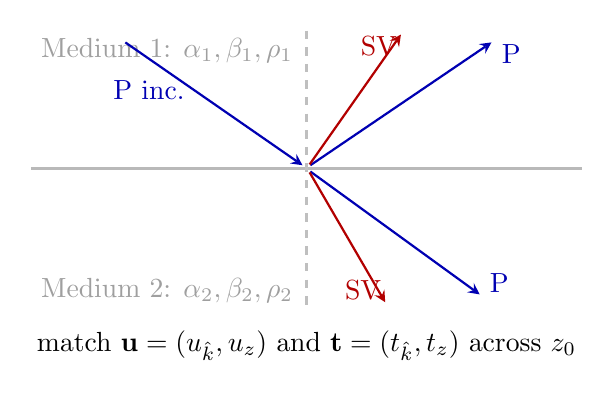
\begin{tikzpicture}[>=stealth, line width=0.8pt]
  \draw[gray!55, line width=1pt] (-3.5,0) -- (3.5,0);
  \draw[gray!50, dashed] (0,1.75) -- (0,-1.75);
  \node[anchor=west, gray!75] at (-3.5,1.5) {Medium 1: $\alpha_1,\beta_1,\rho_1$};
  \node[anchor=west, gray!75] at (-3.5,-1.55) {Medium 2: $\alpha_2,\beta_2,\rho_2$};
  \draw[->, blue!70!black] (-2.3,1.6) -- (-0.05,0.04);
  \node[blue!70!black] at (-2.0,1.0) {P inc.};
  \draw[->, blue!70!black] (0.05,0.04) -- (2.35,1.6);
  \node[blue!70!black] at (2.6,1.45) {P};
  \draw[->, red!70!black] (0.04,0.05) -- (1.2,1.7);
  \node[red!70!black] at (0.92,1.55) {SV};
  \draw[->, blue!70!black] (0.05,-0.04) -- (2.2,-1.6);
  \node[blue!70!black] at (2.45,-1.45) {P};
  \draw[->, red!70!black] (0.04,-0.05) -- (1.0,-1.7);
  \node[red!70!black] at (0.72,-1.55) {SV};
  \node[align=center] at (0,-2.25)
        {match $\mathbf{u}=(u_{\hat k},u_z)$ and $\mathbf{t}=(t_{\hat k},t_z)$ across $z_0$};
\end{tikzpicture}
\caption{Mode conversion at a welded horizontal interface: an incident P wave produces
reflected and transmitted P and SV (SH decouples). The displacement kernels (upper two rows
of $\mathbf{D}$) and traction kernels (lower two rows) are matched across $z_0$; the coupling
entries $\mu C=\rho\omega^{2}-2\mu k^{2}$ and $2\mu k\nu$ drive the conversion.}
\end{figure}

\subsection{Surface impedance and the Rayleigh check}

Write $\mathbf{D}=\big[\begin{smallmatrix}\mathbf{D}_u\\[1pt]\mathbf{D}_t\end{smallmatrix}\big]$,
with $\mathbf{D}_u$ the displacement rows and $\mathbf{D}_t$ the traction rows, and let the
superscript $\downarrow$ select the two columns that decay into a lower half-space
($\mathrm{P}{\downarrow},\mathrm{SV}{\downarrow}$). Eliminating those amplitudes gives the
Dirichlet-to-Neumann (surface-impedance) map $\mathbf{t}=\mathbf{Z}\,\mathbf{u}$,
\begin{equation}
\label{eq:Zimp}
\mathbf{Z}=\mathbf{D}_t^{\downarrow}\big(\mathbf{D}_u^{\downarrow}\big)^{-1}
=\frac{\ii\mu}{k^{2}+\nu_P\nu_S}
\begin{pmatrix}
\kappa_S^{2}\,\nu_P & k\,B\\[2pt]
-\,k\,B & \kappa_S^{2}\,\nu_S
\end{pmatrix},
\qquad B=2k^{2}+2\nu_P\nu_S-\kappa_S^{2},
\end{equation}
with $\mathbf{D}_u^{\downarrow}=\big(\begin{smallmatrix}k&\nu_S\\ \nu_P&-k\end{smallmatrix}\big)$
and $\mathbf{D}_t^{\downarrow}=\big(\begin{smallmatrix}2\ii\mu k\nu_P&\ii\mu C\\
\ii\mu C&-2\ii\mu k\nu_S\end{smallmatrix}\big)$. This $\mathbf{Z}(\kpar,\omega)$ is the traction
kernel in its most usable form: the traction that any prescribed surface displacement must
balance. A traction-free surface of the half-space requires $\det\mathbf{D}_t^{\downarrow}=0$,
that is
\begin{equation}
\big(2k^{2}-\kappa_S^{2}\big)^{2}+4k^{2}\nu_P\nu_S=0
\quad\Longleftrightarrow\quad
\big(2k^{2}-\kappa_S^{2}\big)^{2}=4k^{2}\sqrt{k^{2}-\kappa_P^{2}}\,\sqrt{k^{2}-\kappa_S^{2}},
\end{equation}
the Rayleigh secular function, whose root is the Rayleigh wave. The analogous condition at a
welded solid-solid contact yields the Stoneley wave. Recovering the Rayleigh equation is a
complete check on the P/SV traction kernels.

\subsection{Closing the system}

The single-scatterer response and the host interfaces now live in one basis.
\begin{itemize}
\item \textbf{Free surface and welded interface.} A free surface imposes
$\mathbf{D}_t\,\mathbf{c}=\mathbf{0}$, giving the free-surface reflection matrix
$\mathbf{R}_F=-(\mathbf{D}_t^{\,\mathrm{ref}})^{-1}\mathbf{D}_t^{\,\mathrm{inc}}$. A welded
interface imposes continuity of $\mathbf{D}_u\mathbf{c}$ and $\mathbf{D}_t\mathbf{c}$ across
$z_0$, giving the interface reflection and transmission matrices $\mathbf{R},\mathbf{T}$; SH
closes the same way through $\ii\mu\nu_S$.
\item \textbf{Single-scatterer T-matrix.} On a scatterer boundary the condition is written
through the same displacement and traction kernels: traction-free for a cavity,
displacement-free for a rigid body, continuity of both for a welded inclusion. Projected onto
the partial-wave basis, this yields the scatterer T-matrix $\mathbf{T}_j$.
\item \textbf{The closed system.} With the inter-site structure constants $\mathbf{G}_{ij}$ of
\S4 (intra-plane pieces Ewald-summed) carrying displacement and, through
\eqref{eq:Dmatrix}--\eqref{eq:Zimp}, traction between sites, the self-consistent
multiple-scattering equations are
\begin{equation}
\mathbf{c}_i^{\mathrm{exc}}=\mathbf{c}_i^{0}
+\sum_{j\ne i}\mathbf{G}_{ij}\,\mathbf{T}_j\,\mathbf{c}_j^{\mathrm{exc}},
\qquad i=1,\dots,N,
\end{equation}
or, for a stratified host, the equivalent recursive reflection-transmission addition. The
traction kernels enter twice: in building each $\mathbf{T}_j$, and in matching the host's free
surface and welded interfaces.
\end{itemize}

%==============================================================================
\section{Interplane side scattering and the nearest-neighbour correction}
%==============================================================================

On a space-filling grid of scatterers on the layered background, the convergence theory of
\S2--\S4 dictates a three-way split of the multiple-scattering coupling, the off-diagonal
blocks of the Foldy--Lax system \cite{Foldy1945,Lax1951},
\begin{equation}
\label{eq:split}
G_0^{\text{used}}
=\underbrace{G_0^{\text{intra}}}_{\Delta z=0}
+\underbrace{G_0^{\text{Kennett}}}_{\text{interplane specular}}
+\underbrace{G_0^{\text{side}}}_{\Delta z\neq 0,\ \Delta\brho\neq 0}.
\end{equation}
The same-depth coupling $G_0^{\text{intra}}$ is the spatial near field of \S3, regularised at
coincidence by the cubic-cell T-matrix of \S5. The interplane specular response is carried by
the Kennett reflectivity recursion, exact and unconditionally stable for the layered,
laterally homogeneous part. What the Kennett recursion cannot carry is the lateral momentum
transfer between planes, the scattering $\kpar\to\kpar'$ produced by the lateral heterogeneity
of each plane. That is the interplane side scattering $G_0^{\text{side}}$, the one term the two
clean pieces leave uncovered.

\subsection{The side-scattering kernel}

Between a cell in one plane and a cell in the adjacent plane at vertical offset $h$ and lateral
offset $\Delta\brho$, the direct coupling is the elastic tensor built on $e^{\ii\kappa_c r}/4\pi
r$ with $r=\sqrt{|\Delta\brho|^2+h^2}$, carrying the Kupradze near-field hierarchy
\begin{equation}
\label{eq:sidekernel}
G^{\text{side}}_{ij}\;\sim\;
\frac{A_{ij}(\hat{\mathbf r})}{r}\,e^{\ii\kappa_c r}
\;+\;\frac{B_{ij}(\hat{\mathbf r})}{r^{2}}
\;+\;\frac{C_{ij}(\hat{\mathbf r})}{r^{3}},
\end{equation}
the radiation ($1/r$), intermediate ($1/r^{2}$), and static near-field ($1/r^{3}$) terms. The
$1/r^{3}$ term is excited by the modulus (strain) contrast and dominates at small $ka$; the
$1/r$ term is the displacement coupling of the density contrast. Kennett already carries the
smooth, laterally averaged part of \eqref{eq:sidekernel}; the side correction supplies only the
fluctuation about it.

\subsection{Two ranges, both set by the plane spacing}

That fluctuation is short ranged in two senses, and the same scale $h$ governs both.

\paragraph{Vertically, only adjacent planes.} The interplane coupling at vertical offset $Nh$
carries the evanescent damping $e^{-\kappa_\perp Nh}$ of \eqref{eq:tail} and grows more specular
as its lateral structure washes out with $N$. Distant planes are therefore both damped and
well represented by Kennett; only $N=1$, and marginally $N=2$, needs a side correction.

\paragraph{Laterally, only the first shell.} At fixed $h$ the separation is
$r=\sqrt{|\Delta\brho|^{2}+h^{2}}$, so the near-field terms turn over at $|\Delta\brho|\sim h$.
The dominant $1/r^{3}$ contribution falls between the first diagonal shell ($r=\sqrt2\,h$ at an
edge, $\sqrt3\,h$ at a corner) and the second ($r\approx\sqrt5\,h$) by a factor
$(\sqrt5/\sqrt2)^{3}\approx 4$, so the nearest diagonal neighbours dominate the strain coupling.
Equivalently, the evanescent spectrum that carries the non-specular field is cut at
$k_\parallel\sim 1/h$, whose real-space dual is a kernel of width $\sim h$. For space-filling
cells $h$ is one pitch, and that width is one cell.

The two ranges coincide because they are the same length $h$: the plane spacing that makes the
Kennett recursion converge \emph{between} planes is the spacing that confines the side
scattering \emph{across} them. For space-filling cells the correction is the single shell of
diagonal neighbours, the $4$ edge-sharing cells (lateral offset one pitch) and $4$
corner-sharing cells (offset $\sqrt2$ pitch) in each adjacent plane.

\begin{figure}[h]
\centering
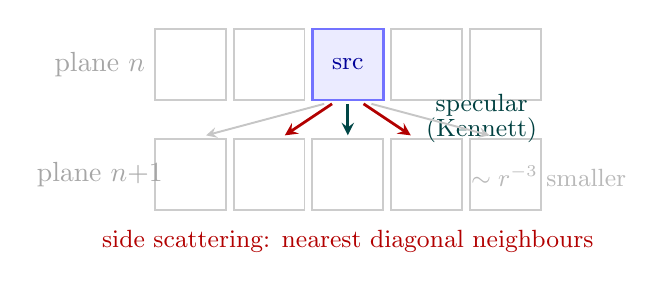
\begin{tikzpicture}[>=stealth, line width=0.7pt]
  \foreach \x in {-2,-1,0,1,2}{
    \draw[gray!40] (\x-0.45,-0.45) rectangle (\x+0.45,0.45);
    \draw[gray!40] (\x-0.45,-1.85) rectangle (\x+0.45,-0.95);
  }
  \draw[blue!55, fill=blue!8, line width=1pt] (-0.45,-0.45) rectangle (0.45,0.45);
  \node[blue!60!black] at (0,0) {\small src};
  \node[gray!70] at (-3.15,0) {plane $n$};
  \node[gray!70] at (-3.15,-1.4) {plane $n{+}1$};
  \draw[->, teal!55!black, line width=1pt] (0,-0.5)--(0,-0.9);
  \node[teal!50!black, align=center] at (1.7,-0.68) {\small specular\\[-3pt]\small (Kennett)};
  \draw[->, red!70!black, line width=1pt] (-0.2,-0.5)--(-0.8,-0.9);
  \draw[->, red!70!black, line width=1pt] (0.2,-0.5)--(0.8,-0.9);
  \node[red!70!black] at (0,-2.25) {\small side scattering: nearest diagonal neighbours};
  \draw[->, gray!45] (-0.3,-0.5)--(-1.8,-0.9);
  \draw[->, gray!45] (0.3,-0.5)--(1.8,-0.9);
  \node[gray!55] at (2.55,-1.42) {\small $\sim r^{-3}$ smaller};
\end{tikzpicture}
\caption{Interplane side scattering on a space-filling grid (cross-section). Kennett carries
the specular vertical coupling; the lateral heterogeneity produces side scattering to laterally
offset cells. The near-field hierarchy confines the missed coupling to the nearest diagonal
shell (offset $\sim h$, one pitch), the second shell being smaller by the $1/r^{3}$ near field.
The directly-below cell is specular and stays in Kennett, so the sparse correction takes only
the diagonal neighbours.}
\end{figure}

\subsection{The sparse correction and its residual}

The side term is then a sparse, banded operator coupling each cell to those $8$ diagonal
neighbours per adjacent plane, evaluated as the volume-averaged spatial propagator and added to
the Kennett recursion. The cost is $O(N)$ with a small constant, and the directly-below cell is
specular and remains in Kennett, so there is no double count. This is the augmented planar
scheme: not pure planar, which drops $G_0^{\text{side}}$, and not full three-dimensional near
field, which pays for all of it, but Kennett plus one shell.

The truncation error of the one-shell correction is the second diagonal shell, governed by the
ratio of the slow $1/r$ (density) coupling to the fast $1/r^{3}$ (modulus) coupling and by
$ka$. In the sub-resonant, modulus-dominated regime the $1/r^{3}$ decay gives a per-shell
factor $\sim 4$ and the correction converges at the first shell; as $ka\to 1$ the $1/r$
radiation term grows and the range lifts. This is the falsifiable content of the
nearest-neighbour hypothesis: a shell-convergence sweep ($0$ shells $=$ pure planar, $1=$
nearest, $2,\dots$) should plateau after the first shell through the Rayleigh-to-moderate
regime, the plateau lifting toward resonance. An empirical companion study measures exactly
that plateau and locates the $ka$ at which a second shell becomes necessary.

\subsection{One stencil for the whole near field}

The range argument of \S7.2 is not special to the interplane term. At $\Delta z=0$ the kernel
\eqref{eq:sidekernel} holds with $r=|\Delta\brho|$, and its $1/r^{3}$ part is equally short
ranged, so the same-depth near coupling is nearest-neighbour dominated as well. The precise
statement, as for the interplane term, is that it is the spatial near \emph{correction} that is
local, not the full same-depth coupling: the long $1/r$ radiation tail of \S2--\S3 does not
truncate, but it is carried by the spectral half, the Ewald-reciprocal sum of \S4, exactly as
the interplane smooth part is carried by Kennett. The two near corrections differ only in which
cheap carrier absorbs their far field.

The entire near field, same-depth and interplane side together, is then a single sparse
real-space stencil over the first three-dimensional shell of the grid (Table~\ref{tab:stencil}).

\begin{table}[h]
\centering
\renewcommand{\arraystretch}{1.3}
\begin{tabular}{@{}lccll@{}}
\toprule
Cells & Count & $(\Delta z,\ |\Delta\brho|)$ & Role & Carried by \\
\midrule
self & $1$ & $(0,\,0)$ & on-site $T_0$ & cubic-cell T-matrix (\S5) \\
vertical faces & $2$ & $(h,\,0)$ & specular & Kennett recursion \\
in-plane ring & $8$ & $(0,\,\{h,\sqrt2\,h\})$ & same-depth near & real-space stencil \\
adjacent diagonals & $16$ & $(h,\,\{h,\sqrt2\,h\})$ & interplane side & real-space stencil \\
remainder & --- & $r\gtrsim\sqrt3\,h$ & smooth far field & spectral propagator \\
\bottomrule
\end{tabular}
\caption{The first three-dimensional shell of the cubic grid and its roles. The self cell is
the solved Eshelby/Galerkin $T_0$; the two vertical faces are specular and ride the Kennett
recursion; the $24$ in-plane and diagonal neighbours are the sparse real-space near correction;
everything beyond is the smooth far field carried by the spectral layered propagator (the
Ewald-reciprocal sum of \S4 with the Kennett $z$-kernel).}
\label{tab:stencil}
\end{table}

Everything collapses to a two-piece operator,
\begin{equation}
\label{eq:twopiece}
G_0=\underbrace{G_0^{\text{near}}}_{\text{24-neighbour real-space stencil}}
+\underbrace{G_0^{\text{far}}}_{\text{global spectral layered propagator}},
\end{equation}
the sparse near correction (volume-averaged, so the strongest coupling, the in-plane
face-sharing neighbour, is represented faithfully) plus the smooth far field carried by the
Ewald-reciprocal / FFT sum with the Kennett reflectivity $z$-kernel. This is the
precorrected-FFT structure of layered-medium integral equations, and the Ewald split of \S4 is
its periodic realisation. The whole development reduces to one rule: solve the first
three-dimensional shell in real space, and everything beyond it in the spectral layered
propagator.

The caveats are uniform across the stencil. It is a $1/r^{3}$, modulus-dominated, small-$ka$
statement; the slow $1/r$ density coupling rides the spectral half; and as $ka\to1$ the
radiation term grows and the shell thickens, at which point the cubes are subdivided and the
scale separation is restored at the finer grid.

%==============================================================================
\section{Adjacent routes and lineage}
%==============================================================================

\begin{itemize}
  \item \textbf{Limiting absorption} is the conceptually cleanest regulator: give $\omega$ a
  positive imaginary part so every $e^{\ii\kappa R}/R$ decays and the real-space sum converges
  absolutely, then continue to real $\omega$. Ewald is how that continuation is realised
  without the cost of literal damping or a slow real-space sum.
  \item \textbf{Singularity subtraction}: subtract the static ($\kappa=0$) lattice sum, whose
  continuation is a known Epstein or Kambe object, and Ewald only the smoother remainder.
  This is useful near lattice resonances, where $\kzG\to 0$ for some order and that term needs
  care.
  \item \textbf{Lineage and references.} Ewald \cite{Ewald1921} for the original split; Kambe
  \cite{Kambe1968} and Ham and Segall \cite{HamSegall1961} for the angular-momentum lattice
  sums of layer-KKR; Linton \cite{Linton2010} for a mathematician-facing survey of Helmholtz
  lattice sums. For the elastodynamic layer-multiple-scattering construction specifically,
  Psarobas, Stefanou and Modinos \cite{Psarobas2000} and Sainidou, Stefanou, Psarobas and
  Modinos \cite{Sainidou2005} carry out exactly the P/S scalar reduction of
  \eqref{eq:opident}. The cleanest write-ups of the dyadic-Ewald bookkeeping live in the
  electromagnetic periodic-Green's-function literature, Capolino, Wilton and Johnson
  \cite{Capolino2007}, and transfer verbatim once the substitution $g_P,g_S$ is made. For the
  elastodynamic and seismological background, Aki and Richards \cite{AkiRichards},
  Kennett \cite{Kennett}, and Ben-Menahem and Singh \cite{BenMenahem}.
\end{itemize}

%==============================================================================
\appendix
\section{The reciprocal half by Poisson summation}
%==============================================================================

With $f(\brho)=e^{-|\brho|^{2}\xi^{2}}$ the two-dimensional Poisson summation formula reads
\begin{equation}
\sum_{\vR\in\Lat}f(\brho-\vR)\,e^{\ii\kpar\cdot\vR}
=\frac{1}{A}\sum_{\vG\in\dLat}\widehat{f}(\kpar+\vG)\,e^{\ii(\kpar+\vG)\cdot\brho},
\qquad
\widehat{f}(\mathbf{k})=\frac{\pi}{\xi^{2}}\,e^{-|\mathbf{k}|^{2}/4\xi^{2}}.
\end{equation}
Insert this into $\mathcal{G}^{(2)}=\tfrac{1}{2\pi^{3/2}}\sum_{\vR}e^{\ii\kpar\cdot\vR}
\int_0^\eta e^{-|\vr-\vR|^{2}\xi^{2}+\kappa^{2}/4\xi^{2}}\,\rd\xi$, use
$|\vr-\vR|^{2}=|\brho-\vR|^{2}+z^{2}$ and
$|\kpar+\vG|^{2}-\kappa^{2}=-\kzG^{2}$, and substitute $\xi\mapsto 1/\xi$ in the radial
integral. At $z=0$ the integral evaluates to
$\int_{1/\eta}^{\infty}e^{\kzG^{2}w^{2}/4}\,\rd w
=\frac{\ii\sqrt{\pi}}{\kzG}\,\erfc(\kzG/2\ii\eta)$,
which delivers \eqref{eq:recip}. As a by-product, $\eta\to\infty$ returns the exact spectral
representation of the periodic Green's function,
\begin{equation}
\mathcal{G}(\brho,z)
=\frac{\ii}{2A}\sum_{\vG\in\dLat}
\frac{e^{\ii(\kpar+\vG)\cdot\brho+\ii\kzG|z|}}{\kzG},
\end{equation}
whose $z=0$ value is the conditionally convergent / divergent sum that motivated the whole
construction.

%==============================================================================
\begin{thebibliography}{99}

\bibitem{Ewald1921} P.~P. Ewald, \emph{Die Berechnung optischer und elektrostatischer
Gitterpotentiale}, Ann. Phys. (Leipzig) \textbf{369}, 253 (1921).

\bibitem{HamSegall1961} F.~S. Ham and B. Segall, \emph{Energy bands in periodic lattices:
Green's function method}, Phys. Rev. \textbf{124}, 1786 (1961).

\bibitem{Kambe1968} K. Kambe, \emph{Theory of low-energy electron diffraction}, Z.
Naturforsch. A \textbf{23}, 1280 (1968).

\bibitem{Linton2010} C.~M. Linton, \emph{Lattice sums for the Helmholtz equation}, SIAM
Review \textbf{52}, 630 (2010).

\bibitem{Psarobas2000} I.~E. Psarobas, N. Stefanou and A. Modinos, \emph{Scattering of
elastic waves by periodic arrays of spherical bodies}, Phys. Rev. B \textbf{62}, 278 (2000).

\bibitem{Sainidou2005} R. Sainidou, N. Stefanou, I.~E. Psarobas and A. Modinos, \emph{A
layer-multiple-scattering method for phononic crystals and heterostructures}, Comput. Phys.
Commun. \textbf{166}, 197 (2005).

\bibitem{Capolino2007} F. Capolino, D.~R. Wilton and W.~A. Johnson, \emph{Efficient
computation of the 2-D periodic Green's function using the Ewald method}, J. Comput. Phys.
\textbf{223}, 250 (2007).

\bibitem{AkiRichards} K. Aki and P.~G. Richards, \emph{Quantitative Seismology}, 2nd ed.,
University Science Books, Sausalito (2002).

\bibitem{Kennett} B.~L.~N. Kennett, \emph{Seismic Wave Propagation in Stratified Media},
Cambridge University Press (1983).

\bibitem{BenMenahem} A. Ben-Menahem and S.~J. Singh, \emph{Seismic Waves and Sources},
Springer, New York (1981).

\bibitem{Thomson1950} W.~T. Thomson, \emph{Transmission of elastic waves through a stratified
solid medium}, J. Appl. Phys. \textbf{21}, 89 (1950).

\bibitem{Haskell1953} N.~A. Haskell, \emph{The dispersion of surface waves on multilayered
media}, Bull. Seismol. Soc. Am. \textbf{43}, 17 (1953).

\bibitem{TakeuchiSaito1972} H. Takeuchi and M. Saito, \emph{Seismic surface waves}, in
B.~A. Bolt (ed.), Methods in Computational Physics, vol.~11, Academic Press, New York (1972),
p.~217.

\bibitem{Foldy1945} L.~L. Foldy, \emph{The multiple scattering of waves}, Phys. Rev.
\textbf{67}, 107 (1945).

\bibitem{Lax1951} M. Lax, \emph{Multiple scattering of waves}, Rev. Mod. Phys. \textbf{23},
287 (1951).

\end{thebibliography}

\end{document}
